\documentclass{vl4}

\begin{document}

\title{Importance of many-body correlations in glass transition:\\an example from polydisperse hard spheres} 

\author{Mathieu Leocmach}
\correspondingauthor{mathieu.leocmach@polytechnique.org}
\affiliation{Laboratoire de Physique, CNRS UMR 5672, Ecole Normale Supérieure de Lyon, 46 allée d'Italie 69364 Lyon cedex 07, France.}
\author{John Russo}
\author{Hajime Tanaka}
\affiliation{ {Institute of Industrial Science, University of Tokyo, 4-6-1 Komaba, Meguro-ku, Tokyo 153-8505, Japan} }

\maketitle

Most of the liquid-state theories, including glass-transition theories, are constructed on the basis of two-body density correlations~\cite{lubchenko2007,Biroli2008,Parisi2010}. 
However, we have recently shown~\cite{tanaka,watanabe_walls,KawasakiJPCM} that many-body correlations, in particular bond orientational correlations, play a key role in both the glass transition and the crystallization transition.

Here~\cite{Leocmach2013a} we show, with numerical simulations of supercooled polydisperse hard spheres systems, that the lengthscale associated with any two-point spatial correlation function does not increase toward the glass transition. A growing lengthscale is instead revealed by considering many-body correlation functions, such as correlators of orientational order, which follows the lengthscale of the dynamic heterogeneities.
Despite the growing of crystal-like bond orientational order, we reveal that the stability against crystallization with increasing polydispersity is due to an increasing population of icosahedral arrangements of particles. 
Our results suggest that, for this type of systems, many-body correlations are a manifestation of the link between the vitrification and the crystallization phenomena.
Whether a system is vitrified or crystallized can be controlled by the degree of frustration against crystallization, polydispersity in this case.  

\begin{figure}
	\centering
	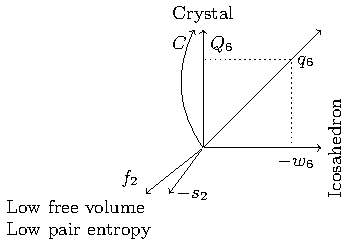
\includegraphics{fig_parameters}
	\caption{Schematic order parameter space considered: $f_2$ and $s_2$ are two-body, $Q_6$ and $C$ are many-body sensitive to crystal-like order, $w_6$ is many-body sensitive to icosahedral order and $q_6$ is many-boy sensible to both crystal-like and icosahedral orders.}
	\label{fig:parameters}
\end{figure}

\begin{figure}[b]
	\centering
	\includegraphics{fig_3D_side}
	\caption{Visualization of the 10\% most ordered particles defined by the various order parameters. All pictures correspond to a thin slice ($5\sigma$) of the same configuration at $\beta p\sigma^3=23$ and $\Delta=7\%$. Only $Q_6$ and $C$ show meaningful spatial fluctuations.}
	\label{fig:3D}
\end{figure}



\begin{acknowledgments}
This study was partly supported by Grants-in-Aid for Scientific Research (S) and Specially Promoted Research from the Japan Society for the Promotion of
Science (JSPS) through its ``Funding Program for World-Leading
Innovative R\&D on Science and Technology (FIRST Program)'' and a JSPS Postdoctoral Fellowship.
ML thank the Region Rhône Alpes and the Programme d'avenir Lyon - Saint Etienne (PALSE NoGELPo) for postoctoral grant.
\end{acknowledgments}


%\bibliography{biblio}
%merlin.mbs apsrev4-1.bst 2010-07-25 4.21a (PWD, AO, DPC) hacked
%Control: key (0)
%Control: author (8) initials jnrlst
%Control: editor formatted (1) identically to author
%Control: production of article title (-1) disabled
%Control: page (0) single
%Control: year (1) truncated
%Control: production of eprint (0) enabled
\begin{thebibliography}{7}%
\makeatletter
\providecommand \@ifxundefined [1]{%
 \@ifx{#1\undefined}
}%
\providecommand \@ifnum [1]{%
 \ifnum #1\expandafter \@firstoftwo
 \else \expandafter \@secondoftwo
 \fi
}%
\providecommand \@ifx [1]{%
 \ifx #1\expandafter \@firstoftwo
 \else \expandafter \@secondoftwo
 \fi
}%
\providecommand \natexlab [1]{#1}%
\providecommand \enquote  [1]{``#1''}%
\providecommand \bibnamefont  [1]{#1}%
\providecommand \bibfnamefont [1]{#1}%
\providecommand \citenamefont [1]{#1}%
\providecommand \href@noop [0]{\@secondoftwo}%
\providecommand \href [0]{\begingroup \@sanitize@url \@href}%
\providecommand \@href[1]{\@@startlink{#1}\@@href}%
\providecommand \@@href[1]{\endgroup#1\@@endlink}%
\providecommand \@sanitize@url [0]{\catcode `\\12\catcode `\$12\catcode
  `\&12\catcode `\#12\catcode `\^12\catcode `\_12\catcode `\%12\relax}%
\providecommand \@@startlink[1]{}%
\providecommand \@@endlink[0]{}%
\providecommand \url  [0]{\begingroup\@sanitize@url \@url }%
\providecommand \@url [1]{\endgroup\@href {#1}{\urlprefix }}%
\providecommand \urlprefix  [0]{URL }%
\providecommand \Eprint [0]{\href }%
\providecommand \doibase [0]{http://dx.doi.org/}%
\providecommand \selectlanguage [0]{\@gobble}%
\providecommand \bibinfo  [0]{\@secondoftwo}%
\providecommand \bibfield  [0]{\@secondoftwo}%
\providecommand \translation [1]{[#1]}%
\providecommand \BibitemOpen [0]{}%
\providecommand \bibitemStop [0]{}%
\providecommand \bibitemNoStop [0]{.\EOS\space}%
\providecommand \EOS [0]{\spacefactor3000\relax}%
\providecommand \BibitemShut  [1]{\csname bibitem#1\endcsname}%
\let\auto@bib@innerbib\@empty
%</preamble>
\bibitem [{\citenamefont {Lubchenko}\ and\ \citenamefont
  {Wolynes}(2007)}]{lubchenko2007}%
  \BibitemOpen
  \bibfield  {author} {\bibinfo {author} {\bibfnamefont {V.}~\bibnamefont
  {Lubchenko}}\ and\ \bibinfo {author} {\bibfnamefont {P.~G.}\ \bibnamefont
  {Wolynes}},\ }\href {\doibase 10.1146/annurev.physchem.58.032806.104653}
  {\bibfield  {journal} {\bibinfo  {journal} {Annu. Rev. Phys. Chem.}\ }\textbf
  {\bibinfo {volume} {58}},\ \bibinfo {pages} {235} (\bibinfo {year}
  {2007})}\BibitemShut {NoStop}%
\bibitem [{\citenamefont {Biroli}\ \emph {et~al.}(2008)\citenamefont {Biroli},
  \citenamefont {Bouchaud}, \citenamefont {Cavagna}, \citenamefont {Grigera},\
  and\ \citenamefont {Verrocchio}}]{Biroli2008}%
  \BibitemOpen
  \bibfield  {author} {\bibinfo {author} {\bibfnamefont {G.}~\bibnamefont
  {Biroli}}, \bibinfo {author} {\bibfnamefont {J.~P.}\ \bibnamefont
  {Bouchaud}}, \bibinfo {author} {\bibfnamefont {a.}~\bibnamefont {Cavagna}},
  \bibinfo {author} {\bibfnamefont {T.~S.}\ \bibnamefont {Grigera}}, \ and\
  \bibinfo {author} {\bibfnamefont {P.}~\bibnamefont {Verrocchio}},\ }\href
  {\doibase 10.1038/nphys1050} {\bibfield  {journal} {\bibinfo  {journal}
  {Nature Phys.}\ }\textbf {\bibinfo {volume} {4}},\ \bibinfo {pages} {771}
  (\bibinfo {year} {2008})}\BibitemShut {NoStop}%
\bibitem [{\citenamefont {Parisi}\ and\ \citenamefont
  {Zamponi}(2010)}]{Parisi2010}%
  \BibitemOpen
  \bibfield  {author} {\bibinfo {author} {\bibfnamefont {G.}~\bibnamefont
  {Parisi}}\ and\ \bibinfo {author} {\bibfnamefont {F.}~\bibnamefont
  {Zamponi}},\ }\href {\doibase 10.1103/RevModPhys.82.789} {\bibfield
  {journal} {\bibinfo  {journal} {Rev. Mod. Phys.}\ }\textbf {\bibinfo {volume}
  {82}},\ \bibinfo {pages} {789} (\bibinfo {year} {2010})}\BibitemShut
  {NoStop}%
\bibitem [{\citenamefont {Tanaka}\ \emph {et~al.}(2010)\citenamefont {Tanaka},
  \citenamefont {Kawasaki}, \citenamefont {Shintani},\ and\ \citenamefont
  {Watanabe}}]{tanaka}%
  \BibitemOpen
  \bibfield  {author} {\bibinfo {author} {\bibfnamefont {H.}~\bibnamefont
  {Tanaka}}, \bibinfo {author} {\bibfnamefont {T.}~\bibnamefont {Kawasaki}},
  \bibinfo {author} {\bibfnamefont {H.}~\bibnamefont {Shintani}}, \ and\
  \bibinfo {author} {\bibfnamefont {K.}~\bibnamefont {Watanabe}},\ }\href@noop
  {} {\bibfield  {journal} {\bibinfo  {journal} {Nature Mater.}\ }\textbf
  {\bibinfo {volume} {9}},\ \bibinfo {pages} {324} (\bibinfo {year}
  {2010})}\BibitemShut {NoStop}%
\bibitem [{\citenamefont {Watanabe}\ \emph {et~al.}(2011)\citenamefont
  {Watanabe}, \citenamefont {Kawasaki},\ and\ \citenamefont
  {Tanaka}}]{watanabe_walls}%
  \BibitemOpen
  \bibfield  {author} {\bibinfo {author} {\bibfnamefont {K.}~\bibnamefont
  {Watanabe}}, \bibinfo {author} {\bibfnamefont {T.}~\bibnamefont {Kawasaki}},
  \ and\ \bibinfo {author} {\bibfnamefont {H.}~\bibnamefont {Tanaka}},\
  }\href@noop {} {\bibfield  {journal} {\bibinfo  {journal} {Nat. Mater.}\
  }\textbf {\bibinfo {volume} {10}},\ \bibinfo {pages} {512} (\bibinfo {year}
  {2011})}\BibitemShut {NoStop}%
\bibitem [{\citenamefont {Kawasaki}\ and\ \citenamefont
  {Tanaka}(2011)}]{KawasakiJPCM}%
  \BibitemOpen
  \bibfield  {author} {\bibinfo {author} {\bibfnamefont {T.}~\bibnamefont
  {Kawasaki}}\ and\ \bibinfo {author} {\bibfnamefont {H.}~\bibnamefont
  {Tanaka}},\ }\href@noop {} {\bibfield  {journal} {\bibinfo  {journal} {J.
  Phys.: Condens. Matter}\ }\textbf {\bibinfo {volume} {23}},\ \bibinfo {pages}
  {194121} (\bibinfo {year} {2011})}\BibitemShut {NoStop}%
\bibitem [{\citenamefont {Leocmach}\ \emph {et~al.}(2013)\citenamefont
  {Leocmach}, \citenamefont {Russo},\ and\ \citenamefont
  {Tanaka}}]{Leocmach2013a}%
  \BibitemOpen
  \bibfield  {author} {\bibinfo {author} {\bibfnamefont {M.}~\bibnamefont
  {Leocmach}}, \bibinfo {author} {\bibfnamefont {J.}~\bibnamefont {Russo}}, \
  and\ \bibinfo {author} {\bibfnamefont {H.}~\bibnamefont {Tanaka}},\ }\href
  {\doibase 10.1063/1.4769981} {\bibfield  {journal} {\bibinfo  {journal} {The
  Journal of Chemical Physics}\ }\textbf {\bibinfo {volume} {138}},\ \bibinfo
  {pages} {12A536} (\bibinfo {year} {2013})},\ \Eprint
  {http://arxiv.org/abs/1211.6819} {1211.6819} \BibitemShut {NoStop}%
\end{thebibliography}%
\end{document}
